\documentclass[]{article}
\usepackage{graphicx}
\graphicspath{ {./} }
%opening
\title{Programming Project - 2}
\author{Dmitry Kalika}

\begin{document}

\maketitle


\section{Introduction}
The primary goal of this project was to implement an algorithm that loads in a set of edges pertaining to a node, and then finds all of its articulation points and biconnected components. In this report, I will discuss articulation points and biconnected components in more detail, the algorithm used to find articulation points and biconnected components, and share the results of running on the algorithm on smaller and larger graphs.
\subsection{Making a Graph} 

I had always assumed that a graph class came as a standard package in python - one that would handle nodes edges (i.e., adding and removing nodes and edges); let you traverse through the graph via dfs or bfs; and plot the graph / results of the traversal. It turns out that a graph class does not come standard in python (though I don't doubt that there are modules available on the internet), so I had to create one.

The graph class I developed can either be initialized as an empty graph, or a .txt file with the format provided in the project description can be used to load in the graph. The graph class has methods to add and remove nodes, add edges. The graph can either be a direct or un-directed graph - this effects the node properties (e.g., connected nodes are both children and parents of each other in an undirected graph). Furthermore, I developed a custom node class that stores various properties of the node such as all of the node's connections, parents, children - whether the node is the root, has been visited, is an articulation point, etc. Before working on this project, I figured that if I wanted to do anything with graphs in python, I would just be able to instantiate a graph type and then proceed with my plan - though I couldn't do that before, I can now do so with my graph class (though I probably want to clean up, comment, and more thoroughly test the robustness of the code before doing so). A quick note if you decide to look through my code: the method named "dfs" is actually an articulation point search using DFS. Initially, the method only did a DFS, but then was modified to find articulation points.

\section{Background}\label(sec:background)
A node is an \textit{articulation point} if the removal of the node results a connected graph to become disconnected. An alternate way to think about this is a "bottle-necked" node, where if you're traversing a graph, you \textbf{have} to go through an articulation point if you want to reach a certain node - there's no alternative path. The lack of an alternative path is the key part to designing an efficient algorithm that finds articulation points - regardless of how we traverse a graph (with a DFS), the discovery time of an articulation point will always be lower than the components "behind" the articulation point. I use the term "behind" a little loosely as it depends on where we begin traversing the graph. For example, Figure A.1 shows that if we start at node A, node D can only be reached if you go through B first, regardless of the direction in which you traverse the graph; therefore, B is bottle-necking the graph. Similarly, if we start at D, a and C will only be reachable if we traverse through B.

\textit{Biconnected components} are a list of edges that make up a sub-graph such that removing any node from the sub-graph will not disconnect the sub-graph. Thus, no articulation points exist in the sub-graph made up of bi-connected components. As described in the previous paragraph, an articulation point creates a bottle-neck such that certain nodes are only reachable when going through the articulation points. Therefore, we simply split up the graph at articulation points, and seperate out regions that are only accessbible through articulation points. In Figure A.1, a graph is shown such that B is the only articulation point, and there are two biconnected components when splitting up the graph at B: (B,D) and (A, B), (A, C), and (B,C).

\subsection{Algorithm Description - Articulation Points}

The most obvious way to search for articulations is to remove a node and see if the graph is still connected; though this would work for small graphs, it requires searching through the entirety of the graph N (\# of nodes) times. Instead, a DFS can be used and the graph only needs to be traversed once. To do this, we must  use what we know about an articulation point:
\begin{enumerate}
	\item If a node (u) is the root of a DFS tree and has at least two children, u is an articulation point. Intuitively, if u is removed, the remaining sub-trees cannot reach one another
	\item If a node (u) has a child (v) that has no back-edge to an ancestor, u is an articulation point. If v does have a back-edge to an ancestor of u, that ancestor is an alternate path to v, and therefore u is not an articulation point.
\end{enumerate}

To discuss the algorithm implemented, lets first introduce two variables that are tracked for each node: discovery time (disc) and low time (low). Discovery time is straightforward - it is simply the time in which the node was first visited / discovered, where every edge takes 1 time unit to travel across. The low time is a little less straightforward, it takes the minimum one of two values for a node u:
\begin{enumerate}
	\item The lowest discovery time of any vertex in a sub-tree rooted by u.
	\item The discovery time of the node that connects the vertex via back-edge.
\end{enumerate}

Case 1 indicates that low(u)$<$disc(v) and there is no-back edge (non-articulation point). Therefore, if low(u)$\geq$disc(v), low must be case 2 indicating a back edge and an articulation point.

\textbf{-- Explain the algorithm in a bit more detail here.}

\subsection{Algorithm Description - Bi-Connected Components}
The algorithm used to find bi-connected components is relatively straight-forward after the articulation point algorithm has been developed. As described in Section 2, bi-connected components are separated by articulation points. The algorithm requires that you keep track of all of the traveled edges as you recursively traverse the graph (using DFS). As you get to the end of the recursion, you add the edge to your stack, and continue adding as you work your way back to the first DFS function call. Whenever an articulation point is discovered, we pop the stack and save all of the edges to a single bi-connected component. It is important to also pop the stack of edges after completing the DFS as we're not guaranteed to have an articulation point at the root, yet the final set of edges still make up a bi-connected component.

\subsection{Implementation Test}
To test the implementation of my articulation point finding algorithm, the graph provided in the programming project description. My algorithm keeps track of both disc, low for each node, as well as whether or not a node is an articulation point. All of these are printed after 'test\_toy\_exp.py' is executed. The console outputs the results shown in Figure \ref{fig:toy}.

\begin{figure}[h]
	\centering
	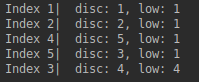
\includegraphics[width=0.4\textwidth]{articulation_ex}
		\caption{simple articulation point example used to test algorithm implementation}\label{fig:toy}
\end{figure}

The results in Figure \ref{fig:toy} are verified by going through the example by hand as shown in Figure A.2. Though it is not shown in the figure, Node 5's articulation property is set to True, thus finding the correct articulation point.

The verification of the bi-connected components finding algorithm is similarly tested on the smaller graph provided in the programming project. Since the only articulation point is node 5, the graph is split into two components such that (5,3) is an edge that makes up a bi-connected component, and then the remaining edges make up the second bi-connected component. As shown in Figure \ref{fig:toy_biconnected}, the implemented algorithm finds the correct bi-connected components.

\begin{figure}[h]
	\centering
	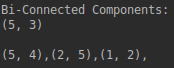
\includegraphics[width=0.4\textwidth]{biconnected_ex}
		\caption{simple articulation point example used to test algorithm implementation}\label{fig:toy_biconnected}
\end{figure}

In addition to the testing performed on the small graph provided in the programming assignment, I tested various graphs that I made up by hand. This really helped me understand the algorithm as well as debug my code. Most of these examples were performed on scratch paper, so they will not be discussed in this report.

\section{Results: Assigned Graph Output}
Now that both algorithms to compute articulation points and bi-connected components have been verified to work (at least on a small-scale problem), we can use the algorithms to compute articulation points and bi-connected components for the assigned graph with 72 graph nodes. The results are shown in Figure \ref{fig:full}.

\begin{figure}[h]
	\centering
	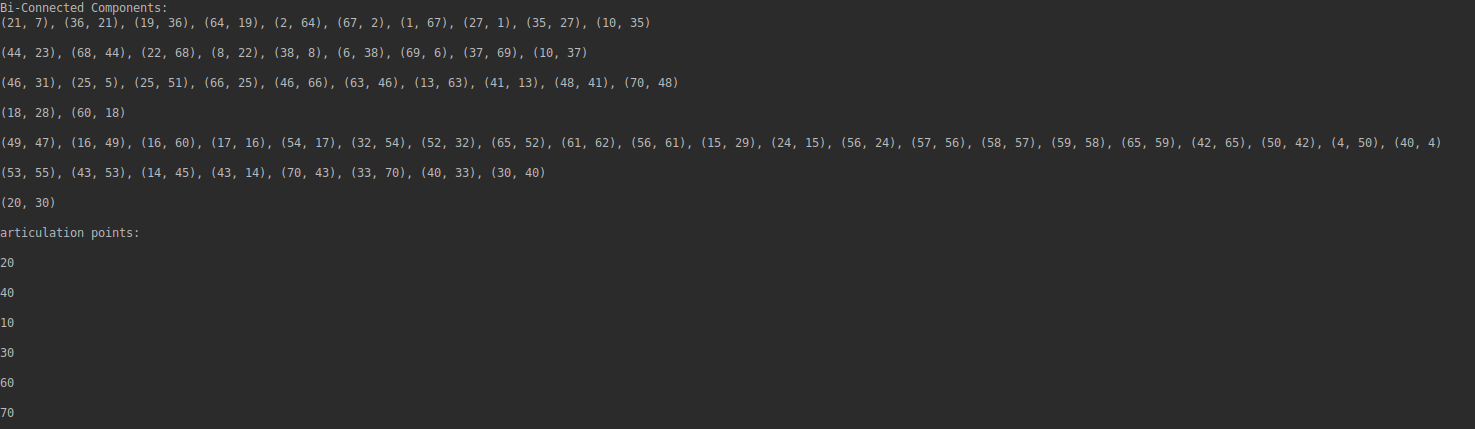
\includegraphics[width=1\textwidth]{full}
		\caption{Articulation and Bi-Connected Components for Assigned Graph}\label{fig:full}
\end{figure}

Prior to assuming that the output is correct, I ran the algorithm with various root nodes to ensure that the outputs of the algorithms agree regardless of which node is used as the root. Regardless of the root node, the outputs were identical, with the only difference being that the articulation points (and thus bi-connected components) were found in different orders.

\section{Conclusion}
In this programming project, I coded up an algorithm that finds articulation points and bi-connected components. Interestingly, I thought I had a really good grasp on how these algorithms worked, until I began the process of coding it up. I quickly realized that some of my intuition was incorrect, and had to alternate between working on the problems by hand, coding up my logic, etc., until the output of my algorithm matched that of the work by hand.

Though I didn't go beyond the scope of the project (i.e., do extra), I spent a great deal of time thinking about all of the interesting ways in which this kind of algorithm (particularly finding articulation points) can be used in practice. One such example I thought about was discovering weak points in complex system architectures. For example, a combat system has many systems communicating with one another; it would be interesting to look at articulation points in a combat system and figure out ways to remove them. The problem would become even more interesting if we consider edge weights that correspond with failure probabilities; for example, if a certain system is unlikely to fail, there's little reason to ensure that the system is not an articulation point, however, a system that is likely to fail should not be an articulation point. Perhaps in this case we would consider the differences between low(u) and disc(v) and set a threshold that indicates a weak node. 

\section{References}
\begin{enumerate}
	\item https://courses.cs.washington.edu/courses/cse421/04su/slides/artic.pdf
\end{enumerate}

\end{document}

